% =====================================================================
%  Workslip — Installationsguide (iOS + Android)
% =====================================================================
\documentclass[8pt,a4paper]{extarticle}

% --- Sprog & tegn ---------------------------------------------------
\usepackage[utf8]{inputenc}
\usepackage[T1]{fontenc}
\usepackage[english]{babel}
\babelprovide[import=da, main]{danish}
\usepackage{lmodern}
\usepackage{textcomp}
\usepackage{microtype}

% --- Layout ---------------------------------------------------------
\usepackage[a4paper,top=8mm,bottom=10mm,left=8mm,right=8mm]{geometry}
\usepackage{xcolor}
\usepackage{graphicx}
\usepackage{tikz}
\usepackage[most,breakable]{tcolorbox}
\usepackage{enumitem}
\usepackage{fontawesome5}
\usepackage{hyperref}
\usepackage{fancyhdr}
\usepackage{lastpage}
\usepackage{ragged2e}

% --- Farver ---------------------------------------------------------
\definecolor{wsBlue}{HTML}{4F6BED}
\definecolor{wsBlueDark}{HTML}{3730A3}
\definecolor{wsInk}{HTML}{1E293B}
\definecolor{wsSlate}{HTML}{475569}
\definecolor{wsSlateLight}{HTML}{94A3B8}
\definecolor{wsInfo}{HTML}{F1F5F9}

% --- Hyperref -------------------------------------------------------
\hypersetup{
  colorlinks=true,
  linkcolor=wsBlueDark, urlcolor=wsBlue,
  pdftitle={Workslip — Installationsguide},
  pdfauthor={Workslip},
  pdfsubject={PWA-installation iOS og Android}
}

% --- Sidefod: side X af Y ------------------------------------------
\pagestyle{fancy}\fancyhf{}
\fancyfoot[C]{\footnotesize\color{wsSlateLight}Workslip \textperiodcentered\ Installationsguide \textperiodcentered\ side \thepage\ af \pageref{LastPage}}
\renewcommand{\headrulewidth}{0pt}\renewcommand{\footrulewidth}{0pt}

% --- Overskrifter: strammet ----------------------------------------
\usepackage{titlesec}
\titleformat{\section}{\color{wsInk}\fontsize{13}{15}\selectfont\bfseries}{}{0pt}{}[{\vspace{0.5mm}\titlerule[1.2pt]\vspace{1mm}}]
\titlespacing*{\section}{0pt}{0pt}{1.5mm}
\titleformat{\subsection}{\color{wsInk}\fontsize{10}{12}\selectfont\bfseries}{}{0pt}{}
\titlespacing*{\subsection}{0pt}{1.5mm}{0.5mm}
\titleformat{\subsubsection}{\color{wsBlueDark}\fontsize{10}{12}\selectfont\bfseries}{}{0pt}{}
\titlespacing*{\subsubsection}{0pt}{2mm}{1mm}

% --- Callouts -------------------------------------------------------
\newtcolorbox{callout}[1][]{
  enhanced, breakable, colback=wsInfo, colframe=wsBlue,
  borderline west={3pt}{0pt}{wsBlue},
  arc=1.5mm, outer arc=1.5mm,
  left=2mm, right=2mm, top=1.5mm, bottom=1.5mm,
  before skip=1mm, after skip=1mm, #1
}
\newcommand{\callouttitle}[1]{{\bfseries\fontsize{7.5}{9}\selectfont\textls[200]{#1}}\par\vspace{0.5mm}}

% --- Step macro: kompakt -------------------------------------------
\newcounter{stepcnt}
\newcommand{\step}[1]{%
  \stepcounter{stepcnt}%
  \par\noindent
\begin{tikzpicture}[baseline=(num.base)]
    \node[circle,fill=wsBlue,text=white,minimum size=5mm,inner sep=0pt,
          font=\bfseries\fontsize{7}{9}\selectfont](num){\arabic{stepcnt}};
  \end{tikzpicture}\hspace{1.5mm}%
  \begin{minipage}[t]{\dimexpr\linewidth-8mm\relax}\RaggedRight #1\end{minipage}\par
  \vspace{0.3mm}
}

% --- Platform-header ------------------------------------------------
\newcommand{\platformheader}[1]{%
  \par\noindent\begin{tcolorbox}[enhanced,breakable,
    colback=wsSlate,coltext=white,
    arc=1.5mm,outer arc=1.5mm,
    left=3mm,right=3mm,top=1.5mm,bottom=1.5mm,
    before skip=0mm,after skip=1mm,halign=left]
    {\fontsize{10}{12}\selectfont\bfseries #1\par}
  \end{tcolorbox}\par
}

% --- List stramning ------------------------------------------------
\setlist[itemize]{leftmargin=4mm,itemsep=0.3mm,topsep=1mm,parsep=0pt}
\setlist[enumerate]{leftmargin=4mm,itemsep=0.3mm,topsep=1mm,parsep=0pt}
\setlength{\parindent}{0pt}
\setlength{\parskip}{0.5mm}
\linespread{1.0}

\begin{document}

\begin{center}
  \begin{tcolorbox}[enhanced,colback=wsInfo,colframe=wsBlue,
    arc=1.5mm,outer arc=1.5mm,
    left=3mm,right=3mm,top=1.5mm,bottom=1.5mm,
    width=\linewidth,halign=center]
  {\normalsize
    \textbf{Installation på iPhone} \textperiodcentered\ \hyperref[sec:android]{Hop til Android-guiden $\rightarrow$}}
  \end{tcolorbox}
\end{center}

\vspace{1mm}

% =====================================================================
% SIDE 1: IPHONE
% =====================================================================
\section{Installation på iPhone}

\setcounter{stepcnt}{0}

\platformheader{iPhone — Safari (anbefalet)}
\subsection{Anbefalet metode}

\step{Åbn \textbf{Safari} (det hvide kompas-ikon).
  \textbf{Ikke} Chrome eller Firefox.}
\step{Indtast dit Workslip-link i adressefeltet og tryk \textbf{Åbn}.}
\step{Tryk på \textbf{Del-ikonet} (\faShareSquare) nederst i Safari.}
\step{Vælg \textbf{"Føj til hjemmeskærm"}.}
\step{Giv den navnet \textbf{"Workslip"} og tryk \textbf{Tilføj}.}
\step{Ikonet ligger nu på din startskærm — tryk for at åbne.}

\bigskip
\noindent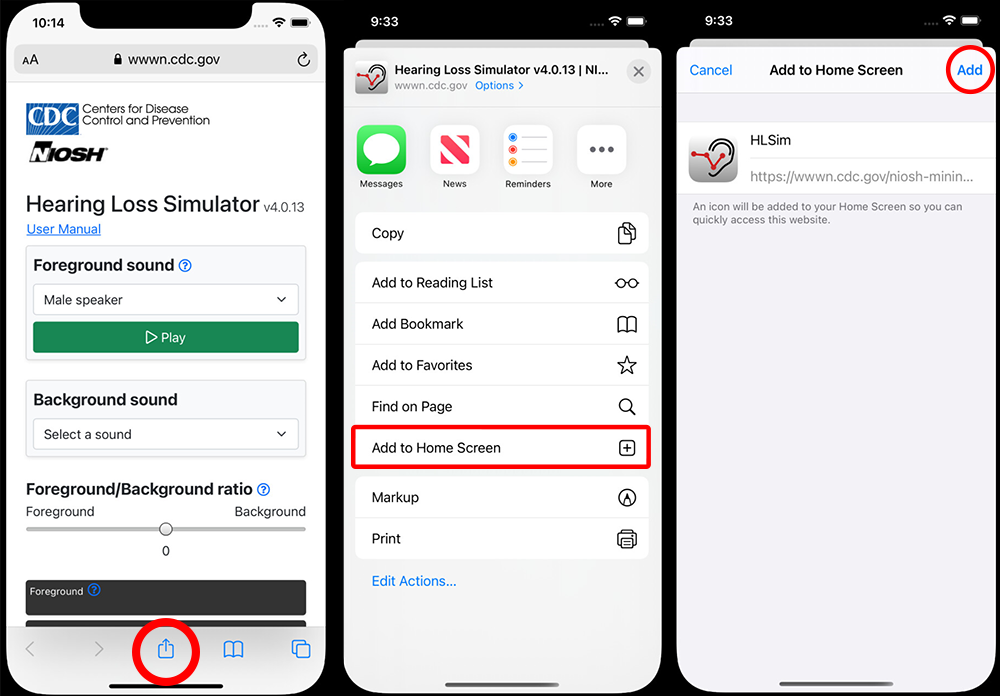
\includegraphics[width=\linewidth]{pwa_ios-safari.png}

\newpage

\platformheader{iPhone — Chrome (alternativ)}
\subsection{Kun hvis du foretrækker Chrome}

\step{Åbn \textbf{Chrome} og indtast dit Workslip-link.}
\step{Tryk på \textbf{Del-ikonet} ($\cdots$ eller firkant med pil).}
\step{Vælg \textbf{"Føj til hjemmeskærm"}, navngiv den \textbf{"Workslip"} og bekræft.}

\bigskip
\noindent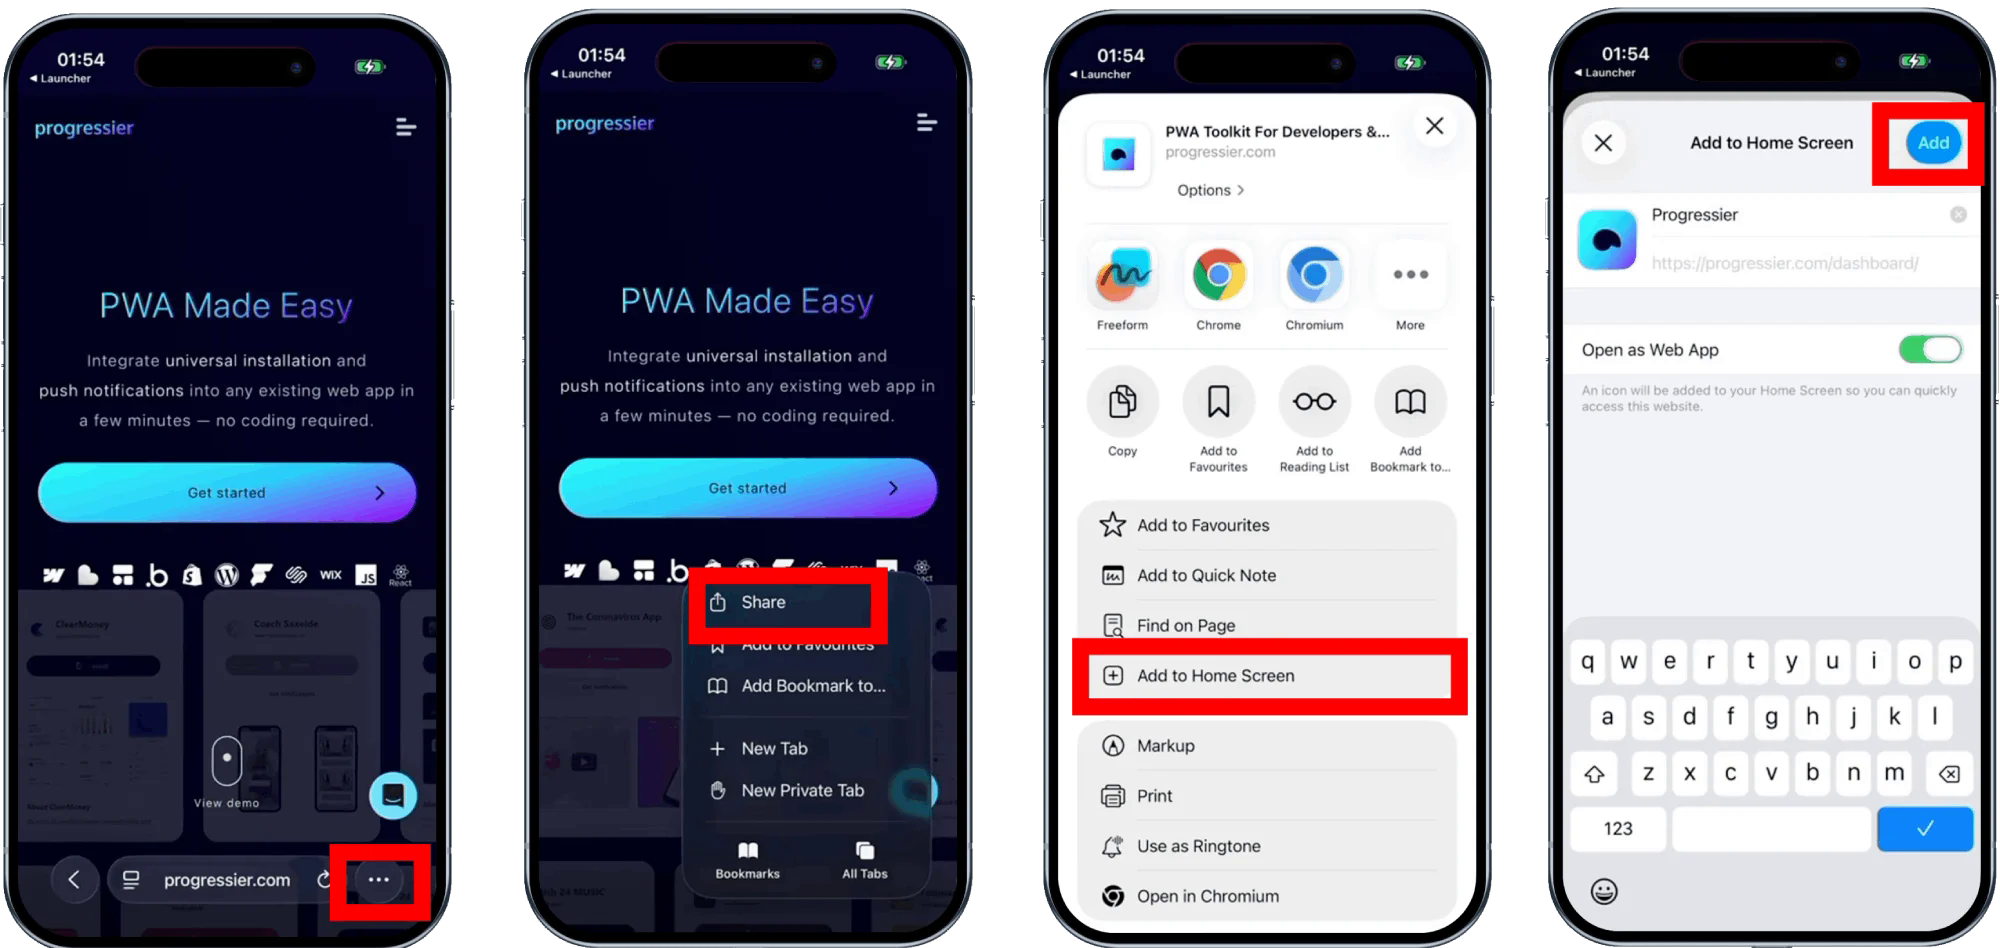
\includegraphics[width=\linewidth]{pwa_ios-chrome.png}
\bigskip

\begin{callout}
\callouttitle{Begrænsning}
Chrome på iPhone understøtter ikke alle PWA-funktioner lige så godt som
Safari. Vi anbefaler Safari — brug kun Chrome hvis du har en god grund.
\end{callout}

\vspace{2mm}
\begin{center}
  \begin{tcolorbox}[enhanced,colback=wsInfo,colframe=wsBlue,
    arc=2mm,outer arc=2mm,
    left=4mm,right=4mm,top=2mm,bottom=2mm,
    width=0.9\linewidth,halign=center]
  {\bfseries\color{wsBlueDark}\large
    \faAndroid\ Har du en Android-telefon? \textperiodcentered\ \hyperref[sec:android]{Hop til Android-guiden $\rightarrow$}}
\end{tcolorbox}
\end{center}

\newpage

% =====================================================================
% SIDE 2: ANDROID
% =====================================================================
\section{Installation på Android}
\label{sec:android}

\setcounter{stepcnt}{0}

\platformheader{Android — Chrome (anbefalet)}
\subsection{Brug "Installer app"-banneret}

\step{Åbn \textbf{Chrome} og indtast dit Workslip-link.}
\step{Tryk på banneret nederst: \textbf{"Tilføj på startskærmen"} (eller \textbf{"Installer app"}).}
\step{Bekræft ved at trykke \textbf{Installer}.}

\bigskip
\noindent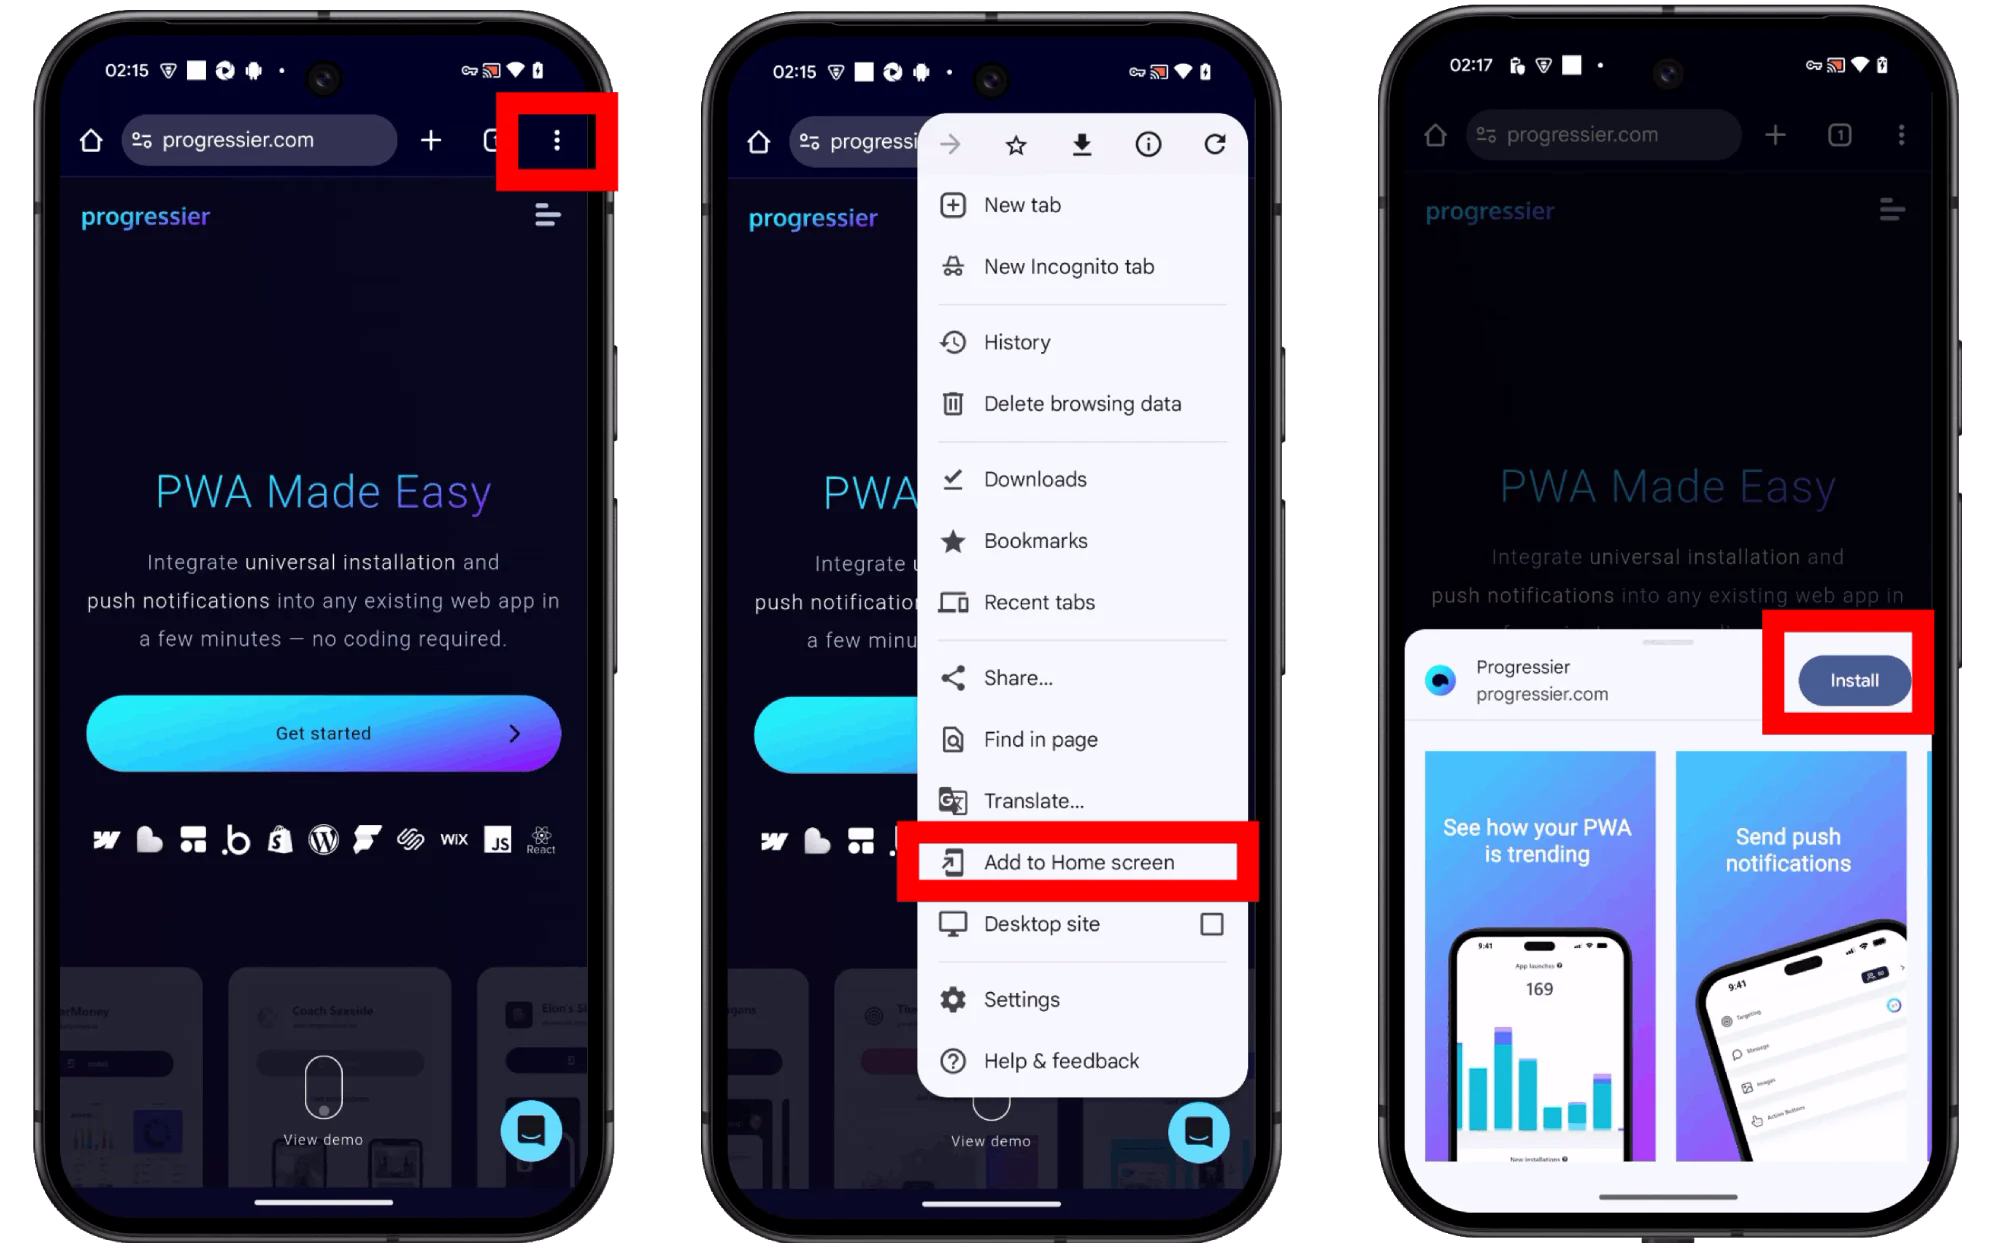
\includegraphics[width=\linewidth]{pwa_android-chrome.png}
\bigskip

\begin{callout}
\callouttitle{Færdig!}
Workslip opdaterer sig automatisk og virker offline, når den har været åbnet med internet én gang.

Visse Android-telefoner viser ikke banneret automatisk — prøv at genindlæse siden eller kontakt support.
\end{callout}

\end{document}
